\clearpage

\begin{appendices}

\begin{figure}[h]
\setlength{\belowcaptionskip}{-5mm}
  \makebox[\textwidth][c]{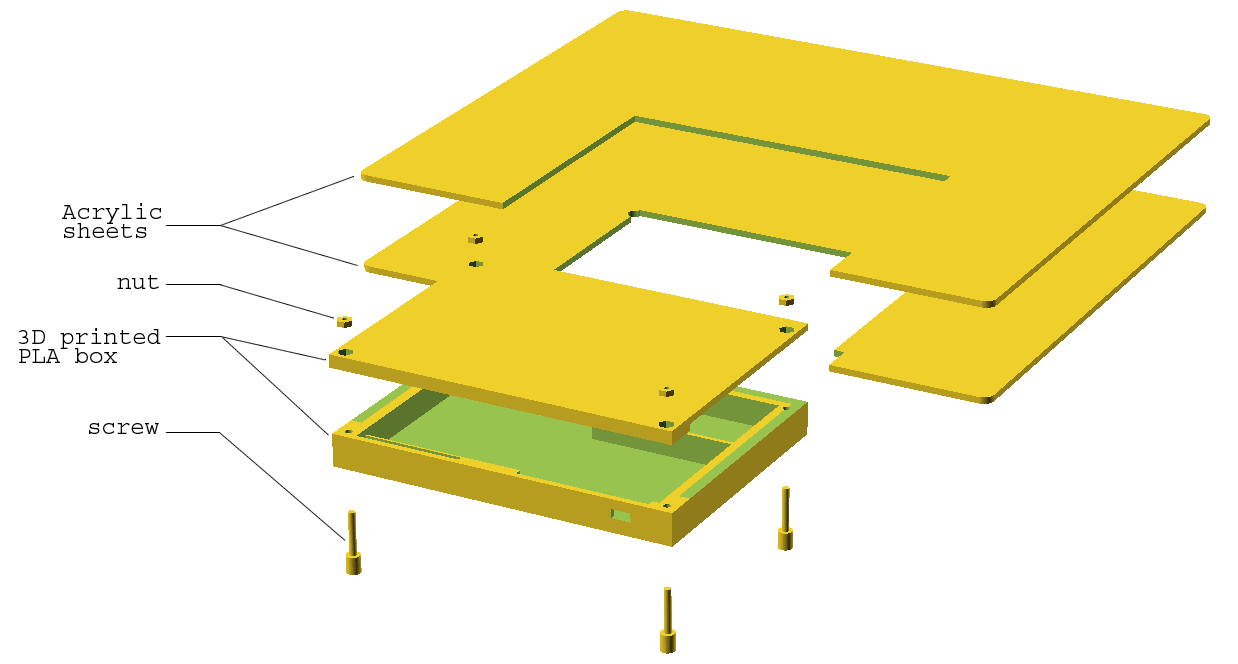
\includegraphics[width=1.2\textwidth]{figures/explode.png}} %
  \caption{\small {\it {Exploded view of the prototype.}}} 
  \label{fig:explode}
\end{figure}

\begin{figure}[h]
\setlength{\belowcaptionskip}{-5mm}
  \makebox[\textwidth][c]{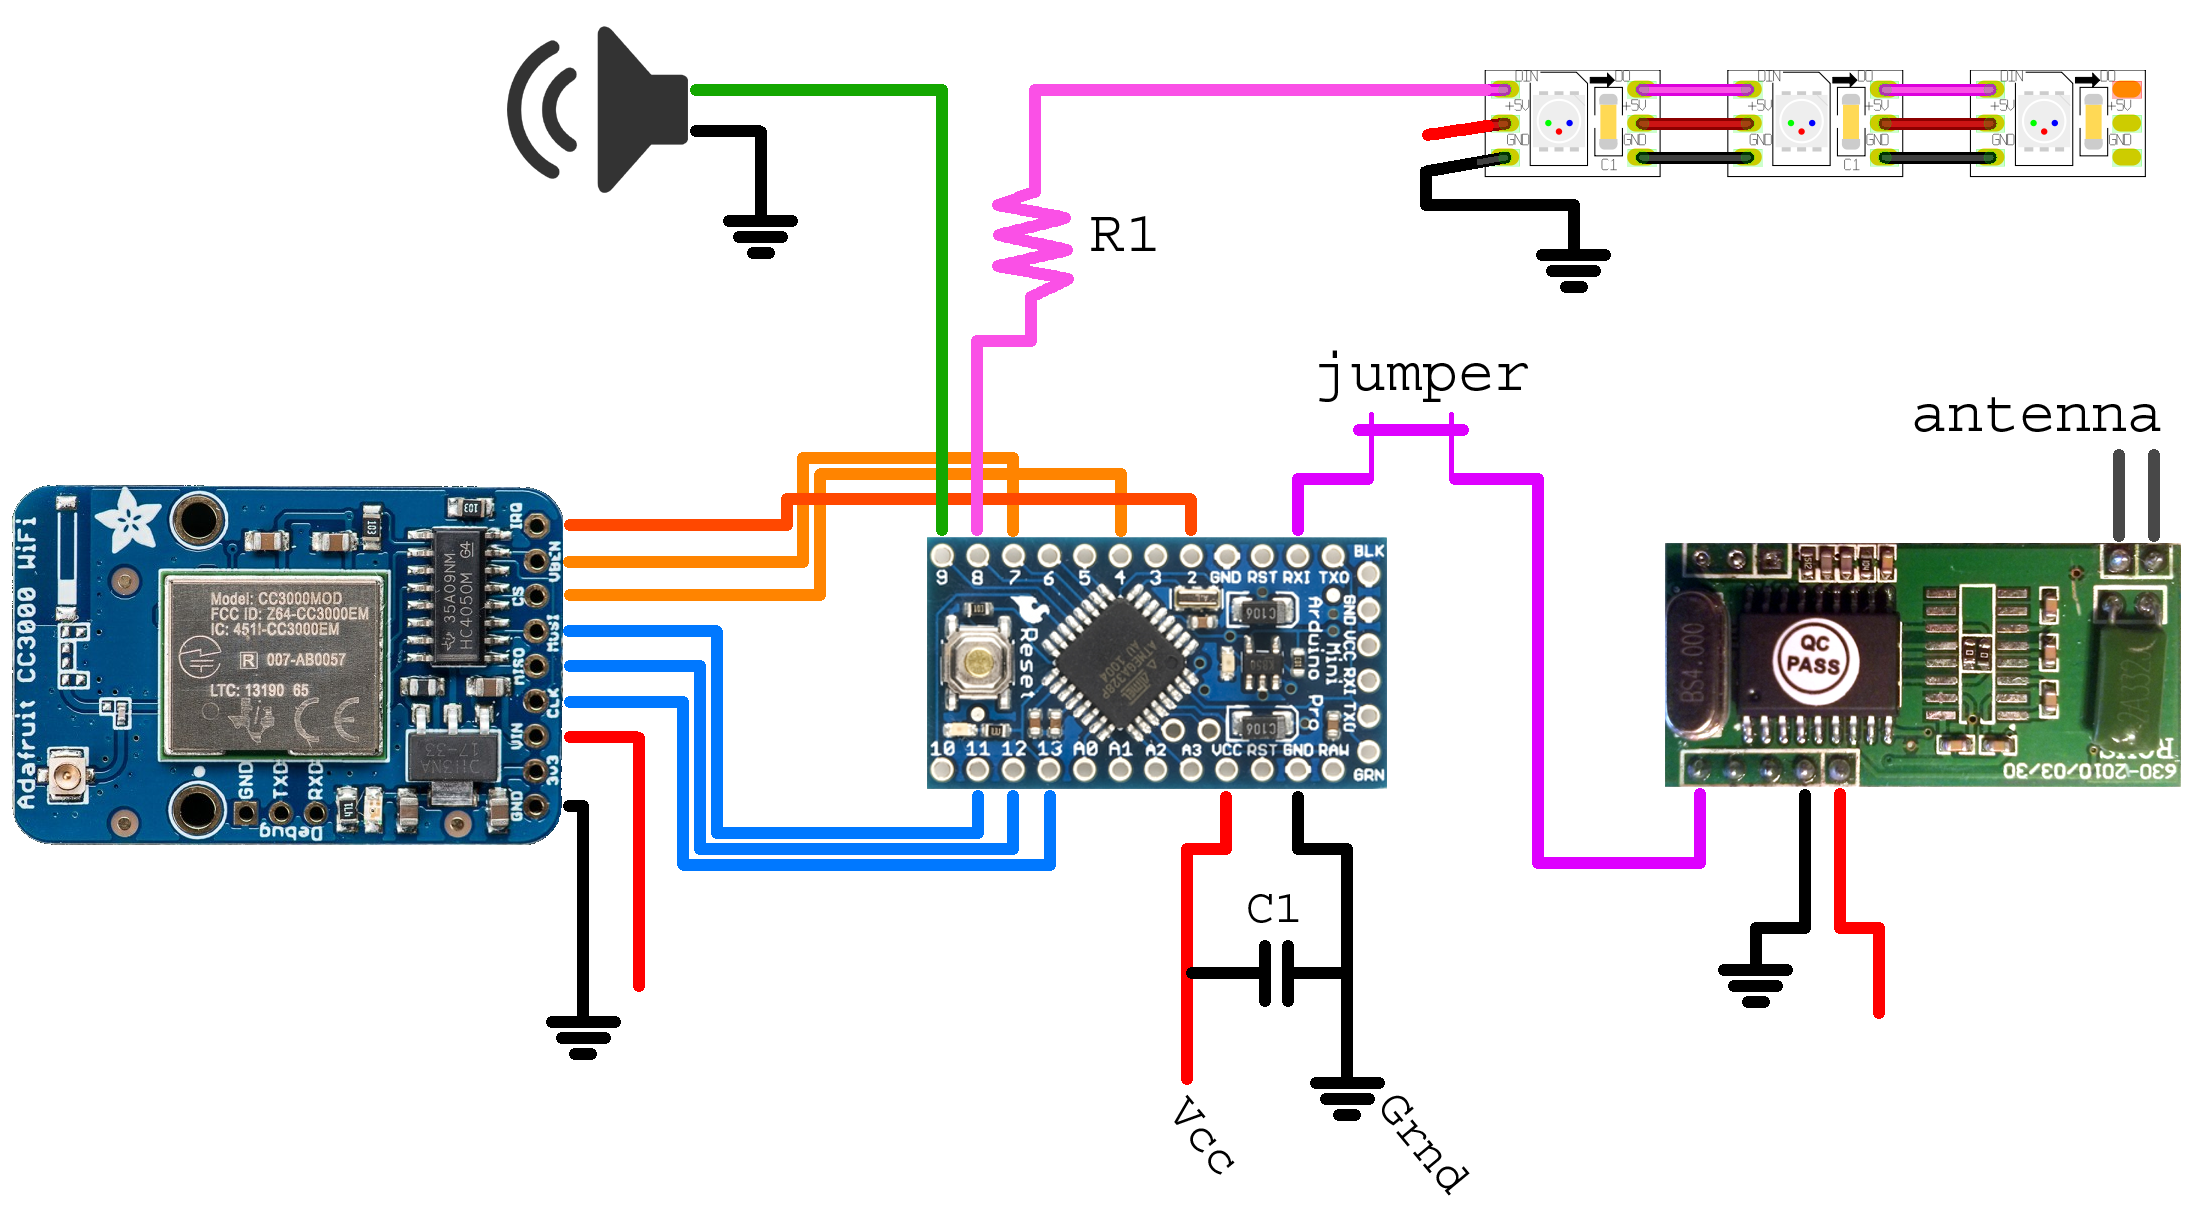
\includegraphics[width=1.2\textwidth]{figures/schematic.png}} %
  \caption{\small {\it {Schematic of the electronics inside.}}} 
  \label{fig:explode}
\end{figure}


\begin{figure}[h]
  \makebox[\textwidth][c]{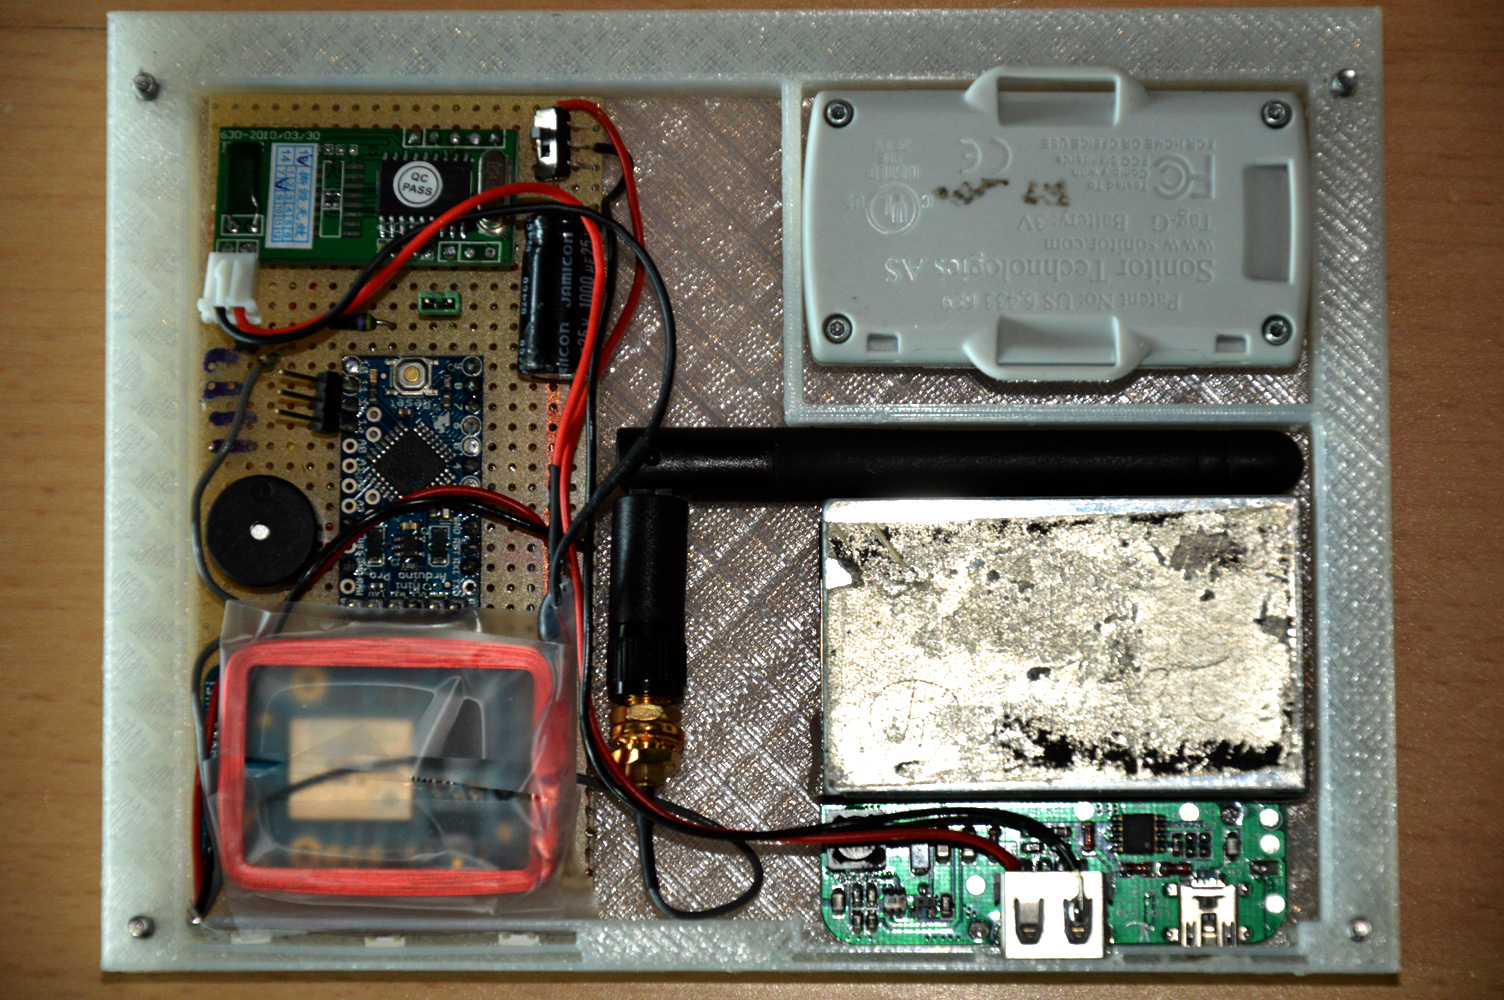
\includegraphics[width=1\textwidth]{figures/internals.jpg}}
  \caption{\small {\it {Inside the electronics compartment.}}} 
  \label{fig:internals}
\end{figure}

\begin{figure}[h]
  \begin{minipage}[b]{.5\textwidth}
    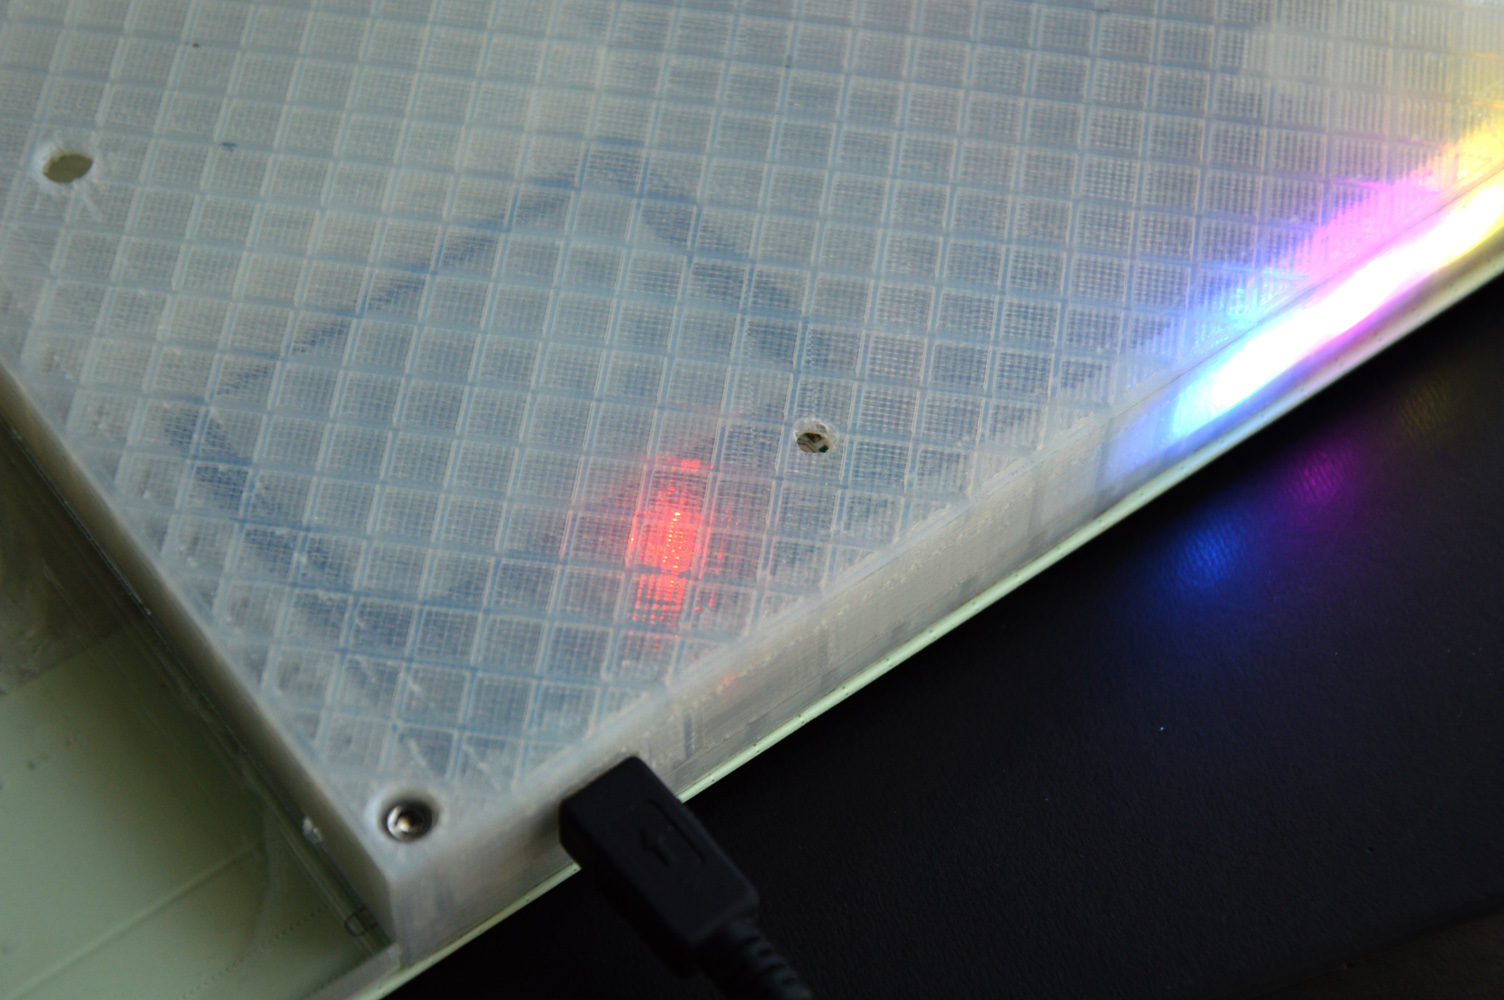
\includegraphics[width=1\textwidth]{figures/journal-charging.jpg}
  \end{minipage}
  \begin{minipage}[b]{.5\textwidth}
    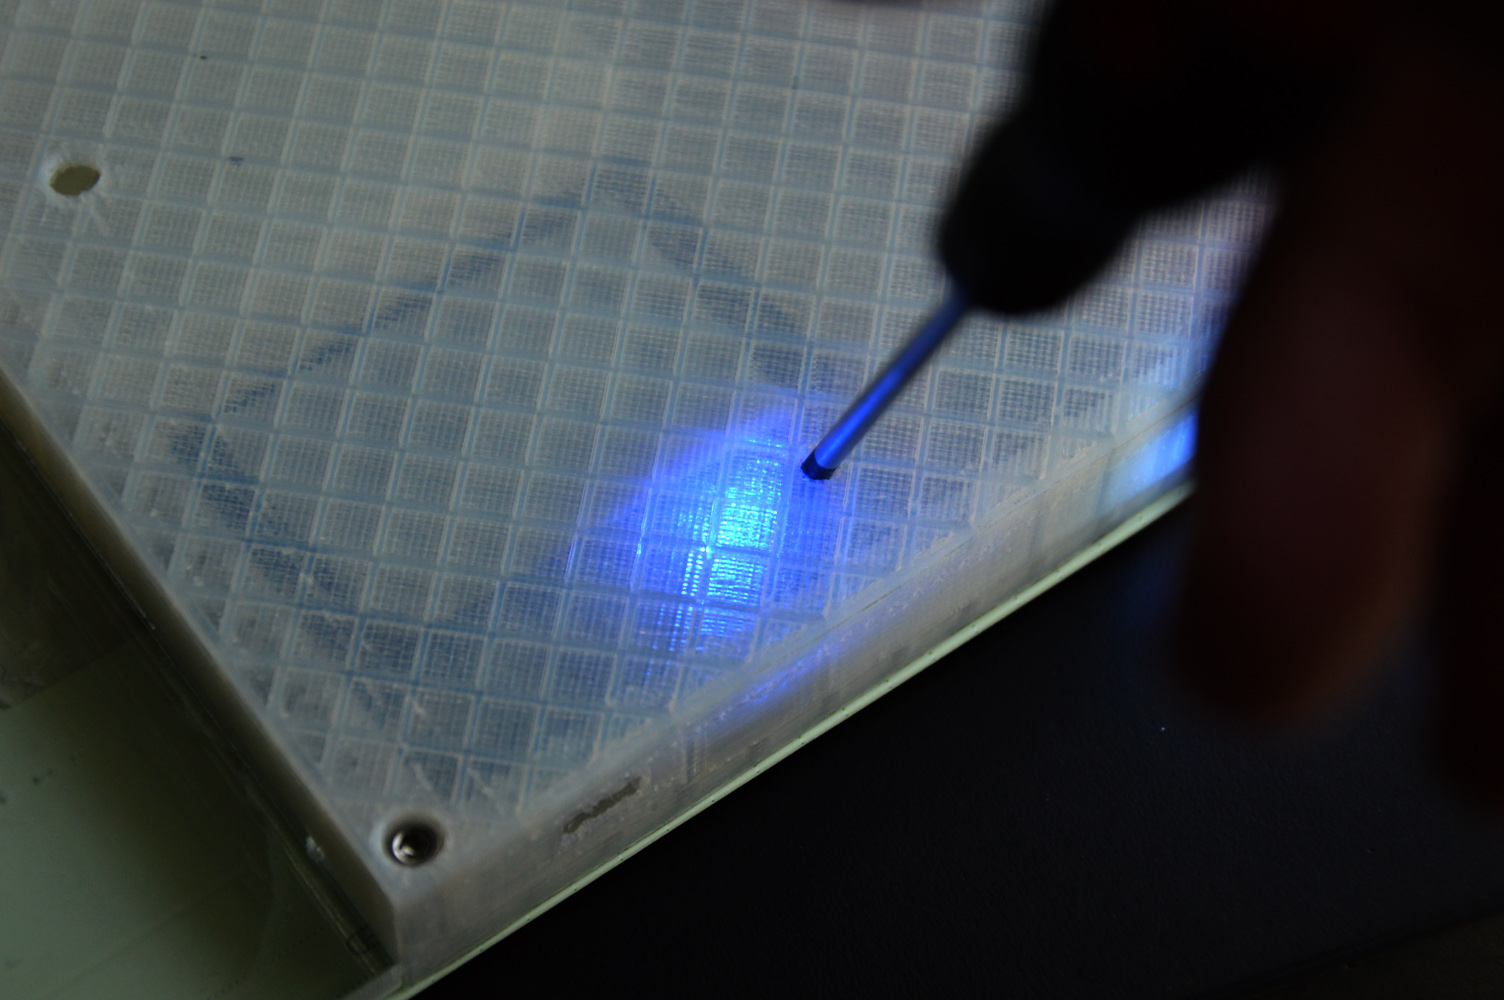
\includegraphics[width=1\textwidth]{figures/journal-battery.jpg}
  \end{minipage}
  \caption{\small {\it {Left: a red LED indicates charging state. Right: a button can be pressed to display battery status.}}}
  \label{fig:journal-2}
\end{figure}

\end{appendices}